% !TEX root = atlas_iros_16.tex
\subsection{Rigid Body and Friction Identification}
\label{sec:advance_ident}
%

%
In our previous work \cite{SpVdTh14} both, rigid body model and friction were simultaneously identified as the parameter vector $\bm{\beta}_{\mathrm{I}}$.
The results still contained a relevant error regarding model fitting and plausibility of the friction parameters compared to single-joint experiments.
Therefore, in this work a sequential procedure was applied, where pre-identified Coulomb and viscous friction parameters $\bm{d}_\mathrm{v,p}$, $\bm{\mu}_\mathrm{C,p}$ were included into the identification procedure in order to reduce the parameter space from $59$ to $45$
unknowns\footnote{
The 70 dynamic parameters (10 per joint) are reduced to $n_\mathrm{b}=45$ in the minimal regressor form.
Additionally, the model has $2n_\mathrm{j}=14$ friction parameters (2 per joint) resulting in $n_\beta=59$ parameters overall, see \cite{SpVdTh14}.}.
\subsubsection{Identification Model and Approach}
%
For identification purposes the robot dynamics (\ref{eqn:invdyn}), including a suitable friction model, can be written in regressor form as  
\begin{equation}
\bm{\tau}_{\mathrm{m}} = \bm{\Phi} \bm{\beta} - \bm{\tau}_{\mathrm{ext}},
\label{regressor}
\end{equation}
where the regressor matrix $\bm{\Phi}$ contains distinct base and friction parameter related columns $\bm{\Phi} = \begin{pmatrix} \bm{\Phi}_\mathrm{b} & \bm{\Phi}_\mathrm{f} \end{pmatrix}$. 
The elements of the parameter vector $\bm{\beta} = \begin{pmatrix} \bm{\beta}_\mathrm{b} \ \bm{d}_\mathrm{v} \ \bm{\mu}_\mathrm{c} \end{pmatrix}^{\mathrm{T}}$ denote the base, viscous friction and Coulomb friction parameter vectors. 
The regressor matrix of the friction model can be allocated as 
\begin{equation}
\bm{\Phi}_\mathrm{f}(\dot{\bm{q}}) =   
\begin{pmatrix}
\mathrm{diag}\{\dot{\bm{q}}\}& 
\mathrm{diag}\{\mathrm{sgn}(\dot{\bm{q}})\}\\
\end{pmatrix}.
\label{friction_mdl}
\end{equation} 
Assuming $\bm{\tau}_{\mathrm{ext}} = \bm{0}$ during identification procedure, the influence of (\ref{friction_mdl}) can be incorporated by subtracting (\ref{friction_mdl}) from both sides in (\ref{regressor}).
This leads to the friction-corrected motor torque
\begin{align}
\bm{\tau}_{\mathrm{m},\mathrm {f}} &= 
\bm{\tau}_{\mathrm{m}} -  \bm{\Phi}_{\mathrm{f}} ( \dot{\bm{q}})(\bm{d}_{\mathrm{v}}, \bm{\mu}_{\mathrm{c}})^{\mathrm{T}}\\ 
&=
\bm{\Phi} \bm{\beta} - \bm{\Phi}_{\mathrm{f}} ( \dot{\bm{q}})(\bm{d}_{\mathrm{v}}, \bm{\mu}_{\mathrm{c}})^{\mathrm{T}}=\bm{\Phi}_\mathrm{b}\bm{\beta}_\mathrm{b}.
\end{align}
%TODO QUELLE
%The influence of friction to motor torque $\bm{\tau}_{\mathrm{m}}$ can now be corrected by $\bm{\tau}_{\mathrm{m},\mathrm {f}} = \bm{\tau}_{\mathrm{m}} - \bm{\Phi}_{\mathrm{f}} ( \dot{\bm{q}})(\bm{d}_{\mathrm{v}}, \bm{\mu}_{\mathrm{c}})^{\mathrm{T}}$ using prior knowledge of friction parameters $\bm{d}_\mathrm{v,p}$ and $\bm{\mu}_\mathrm{c,p}$. 
Identifying the numerical values of $\bm{\beta}_{\mathrm{b}}$ is done using a Moore-Penrose pseudoinverse 
%
\begin{equation}
\hat{\bm{\beta}}_{\mathrm{b}} = {\left( \bm{F}^{\mathrm{T}} \bm{\Sigma}^{-1} \bm{F} \right)}^{-1}  \bm{F}^{\mathrm{T}} \bm{\Sigma}^{-1}\bm{b}
\label{MoorePenrose}
\end{equation}
%
filled with experimentally gained optimized Fourier-based joint angle trajectories of duration $t_{\mathrm{f}}$ \cite{park2006fourier}. 
The information matrix $\bm{F}$ and the measurement vector $\bm{b}$ are defined as
%
\begin{equation}
\bm{F} = \begin{pmatrix}
\bm{\Phi}_{\mathrm{b}}\left( \bm{q}(t_1),\dot{\bm{q}}(t_1),\ddot{\bm{q}}(t_1) \right) \\
\bm{\Phi}_{\mathrm{b}}\left( \bm{q}(t_2),\dot{\bm{q}}(t_2),\ddot{\bm{q}}(t_2) \right) \\
\vdots \\
\bm{\Phi}_{\mathrm{b}}(\bm{q}(t_{\mathrm{f}}),\dot{\bm{q}}(t_{\mathrm{f}}),\ddot{\bm{q}}(t_{\mathrm{f}}))\end{pmatrix},~~
\bm{b} = \begin{pmatrix}
\bm{\tau}_\mathrm{m,f}(t_1) \\
\bm{\tau}_\mathrm{m,f}(t_2) \\
\vdots \\
\bm{\tau}_\mathrm{m,f}(t_{\mathrm{f}})
\end{pmatrix},
\end{equation}
%
where $\bm{\tau}_\mathrm{m,f}(t_i)$ are friction-corrected torque measurements using prior knowledge of friction parameters $\bm{d}_\mathrm{v,p}$ and $\bm{\mu}_\mathrm{c,p}$.
The covariance matrix $\bm{\Sigma}$ is composed of actuator noise variances.
Torque measurements $\bm{\tau}_{\mathrm{m}}$ are determined based on chamber pressures for the hydraulic joints and electric currents for the electromechanic joints.
Gear ratios and motor constants are provided by the manufacturer.
The joint angle $\bm{q}$ is measured by position encoders. 
The resulting parameter vector $\bm{\beta}_{\mathrm{II}}$ of the sequential method, which is used to parameterize (\ref{regressor}), consists of the elements $\bm{\beta}_{\mathrm{II}} = \begin{pmatrix} \bm{\beta}_\mathrm{b} \ \bm{d}_\mathrm{v,p} \ \bm{\mu}_\mathrm{c,p} \end{pmatrix}^{\mathrm{T}}$.

\subsubsection{Single Joint Friction Identification}

The identification of joint friction parameters $\bm{d}_{\mathrm{v,p}}$ and $\bm{\mu}_{\mathrm{c,p}}$ is done by running a set of different constant velocities $\dot{q}_i$ in positive and negative direction and measuring the resulting torque $\bm{\tau}_{\mathrm{m}}$ for every joint. 
Mean velocity and torque are calculated using intervals of constant speed.
Figure~\ref{fig:ident_friction_char} depicts the joint friction characteristics for the hydraulic joints which show significant Coulomb and viscous friction. 

% figure generated with MATLAB in
% drc_paper/Atlas_IROS_16/figures/Identification/FrictionCharacteristics_resultfigures_IROS.m
\begin{figure}
\centering
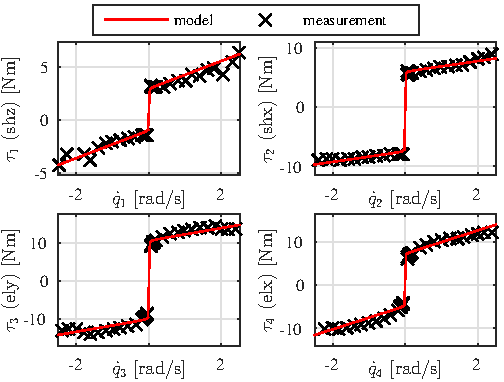
\includegraphics[]{./figures/Identification/FrictionCharacteristics_left}
\caption{Viscous and Coulomb friction for the hydraulic joints of the left arm. Each marker represents the mean value of one constant velocity single joint experiment, see Fig.~\ref{fig:velocity_tracking_friction}. Dynamics effects from $\bm{\Phi}_{\mathrm{b}}$ were removed and calculated with dynamics parameters $\hat{\bm{\beta}}_{\mathrm{b,I}}$ from the combined identification approach \cite{SpVdTh14} and with assumed fixed and upright upper body orientation.}
\label{fig:ident_friction_char}
\SkipBeforePicture
\end{figure}

The identification results could be further improved by using the impedance controller to execute the identification trajectory, as it shows significantly improved velocity tracking compared to an extensively tuned PD controller implemented by the manufacturer, see Fig.~\ref{fig:velocity_tracking_friction}.
The identified friction parameters are given in Table~\ref{tab:errors_tracking_left}.

%
% figure generated with MATLAB in
%./figures/Identification/ConstVel_AssemblyFigure_middle_plot.m
\begin{figure}
\centering
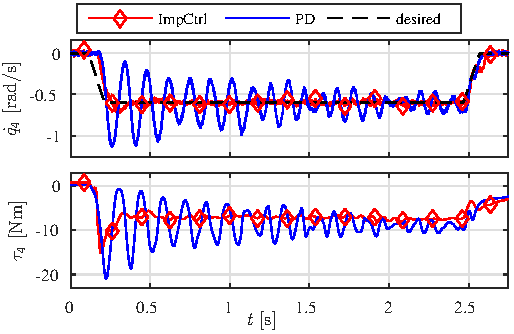
\includegraphics[width=\linewidth]{./figures/Identification/SI_E036_Joint4_ConstVel_Summary_medium_speed}
\caption{Single joint friction experiment exemplified for joint 4 reveals improved velocity tracking of the impedance controller compared to PD position control with controller gains from \cite{2014:JFR-ViGIR-DRC-Trials, ConnerKohRomStu2015}.}
\label{fig:velocity_tracking_friction}
\SkipBeforeText
\end{figure}

% MSE-Werte werden auch in atlas5_plot_torque_ident_MPV_left_DRC_IROS.m ausgegeben.
%
\setlength\tabcolsep{5pt}
\begin{table}
   \caption{Mean square errors (MSE) for arm identification using different base parameter vectors $\hat{\bm{\beta}}_{\mathrm{I}}$, $\hat{\bm{\beta}}_{\mathrm{II}}$ and data from Fig.~\ref{fig:ident_torque_compare} and identified friction parameters from single-joint experiments}
  \begin{center}
   \begin{tabular}{c|c|c|c|c}
joint  & $\mathrm{MSE}(\bm{\tau}_{\mathrm{m}}-\bm{\tau}_{\mathrm{I}})$   & $\mathrm{MSE}(\bm{\tau}_{\mathrm{m}}-\bm{\tau}_{\mathrm{II}})$   & $\hat{{\mu}}_{\mathrm{C,p},i}$ & $\hat{{d}}_{\mathrm{v,p},i}$ \\
 & [(Nm)$^2$] & [(Nm)$^2$] & [Nm] & [Nms/rad] \\ 
\hline
1 (shz) &  97.04  & 13.03 & 2.0 & 1.3 \\
2 (shx) &  52.64  & 20.78 & 6.7 & 0.9 \\
3 (ely) &  22.58  & 16.62 & 10.3 & 1.6 \\
4 (elx) &  25.22  & 18.66 & 6.1 & 2.7 \\
\hline
5 (wry) &  2.82 & 6.50 & 0.1 & 0.5 \\
6 (wrx) &  8.11 & 3.46 & 0.1 & 0.2 \\
7 (wry2) &  0.26 & 18.28 & 3.1 & 0.2 \\
   \end{tabular}
  \end{center} 
\label{tab:errors_tracking_left}
\SkipBeforePicture
\end{table}
\setlength\tabcolsep{6pt}

\subsubsection{Results of the Sequential Identification}

A comparison between the base parameter vector $\hat{\bm{\beta}}_{\mathrm{I}} = \begin{pmatrix} \hat{\bm{\beta}}_\mathrm{b,I} \ \hat{\bm{d}}_\mathrm{v} \ \hat{\bm{\mu}}_\mathrm{C} \end{pmatrix}^{\mathrm{T}}$, where friction was identified as part of the combined least squares optimization \cite{SpVdTh14}, and the base parameter vector $\hat{\bm{\beta}}_{\mathrm{II}}$ of the sequential method can be found in Fig.~\ref{fig:ident_torque_compare}.
Good model consistency is indicated by low distance between model and measurement.
To avoid the problem of overfitting, the trajectory of this experiment was different from the one used for identification.
When using the parameter vector $\hat{\bm{\beta}}_{\mathrm{II}}$, significantly improved results could be achieved in the hydraulic joints, indicated by the lower mean square error between measured and modeled torques in Table~\ref{tab:errors_tracking_left}.

% Bildquelle: atlas5_plot_torque_ident_MPV_left_DRC_IROS.m
\begin{figure}
\centering
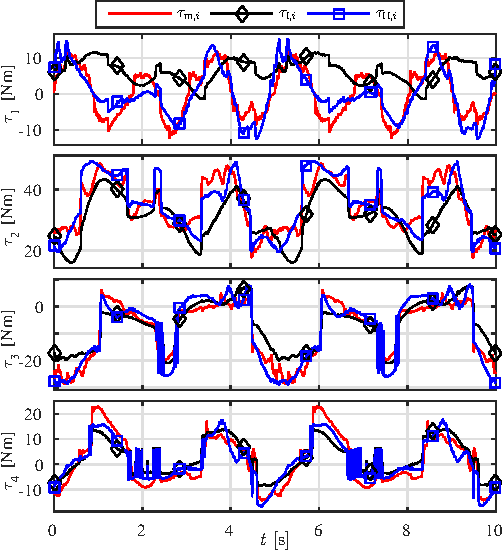
\includegraphics{./figures/Identification/atlas5_plot_torque_ident_MPV_left_IROS}
\caption{Measured ($\bm{\tau}_\mathrm{m}$) and simulated torques of the left arm joints comparing the sequential method $\bm{\tau}_{\mathrm{\mathrm{II}}}$ with the combined method $\bm{\tau}_{\mathrm{\mathrm{I}}}$.}
\label{fig:ident_torque_compare}
\SkipBeforeText
\end{figure}

As already mentioned in \cite{SpVdTh14}, the electromechanic wrist joints (wry, wrx, wry2) do not seem to be identifiable for the Atlas system without working joint torque sensors.
Although friction was identified in single axis experiments, the predicted
torques have essentially no correlation with the measured torques. 
Presumably, this is due to the current-based torque measurement on actuator side, which decreases the quality of the measured information significantly.

In the next section, the results for the experimental collision handling performance with the Atlas system are outlined. 